\newpage
\section{Introduction}
\label{sec:introduction}

\paragraph{} The main objective of this laboratory assignment is to develop a circuit that 
convert a AC sinal (230V) to a DC sinal (with 12V), so we choose one architecture for the Envelope Detector 
and Voltage Regulator to be able to have that.
 We decided to separate this work in three different sections. \paragraph{}
In the first one, using Ngspice tools, in the second section Simulation \ref{sec:simulation}, we will present a 
simulation of the circuit. Then, in Theoretical Analysis \ref{sec:analysis}, we present a suitable theoretical
model able to predict the output of the Envelope Detector and the Voltage Regulator circuit. We also explain 
the reason of each component that we used in the circuit.
\paragraph{}Finally, we put the graphs side by side and compare it and explain the differences.
 \paragraph{}Lastly, Conclusion \ref{sec:conclusion}, the contents of the report will be summarised and the 
achieved results discussed.

\paragraph{} We decided to use the circuit below. The reason why this circuit was chosen is explained later.

\begin{figure}[h]
    \centering
    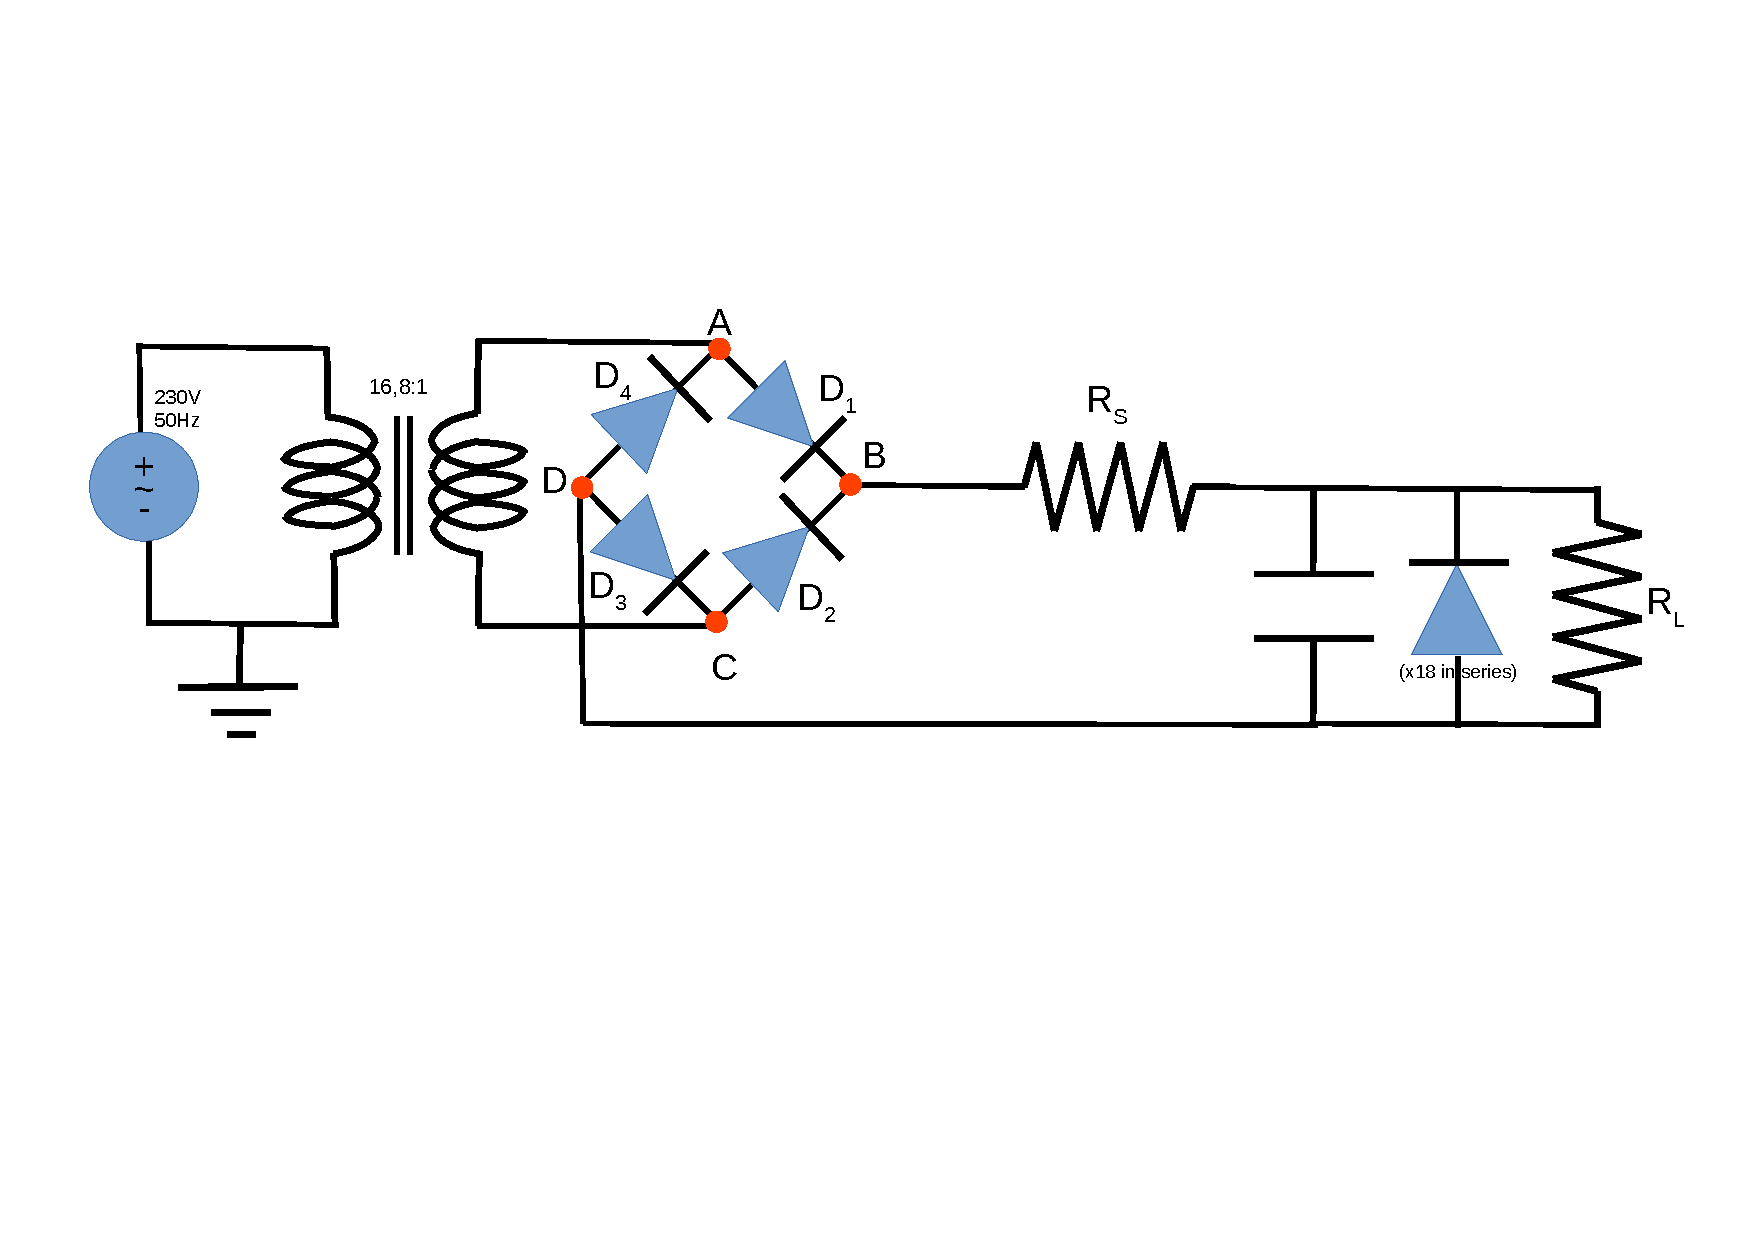
\includegraphics[width=0.8\linewidth]{circuit.pdf}
    \caption{Circuit}
    \label{fig:circuit}
\end{figure}
